\section{Experimental validation}\label{sec:experiments}

\todo[inline]{WIP}

In this section, we validate the utility of the CLEAVE framework through scalability measurements of a networked control system running on a WiFi link.
We aim to answer questions about the ability of CLEAVE to provide relevant and accurate metrics on the performance of such setups as \emph{system load} increases.
In this context, we will focus on the load as it manifests on the network link in terms of the reliability of the link and the associated latencies. 
We adopt this constrained view of load due to the characteristics of NCS, where controllers are usually relatively lightweight in terms of computing resources, leaving the network link as the principal bottleneck in the system.

Our experimental setup is depicted in \cref{fig:cleave:expsetup}.
A number between 1 and 12 of CLEAVE Plants running on dedicated light-weight general purpose computing devices (in this case, Raspberry Pi 4's) connect wirelessly to an 802.11n WiFi Access Point (AP).
This AP in turn connects via Ethernet to a host on which the CLEAVE Dispatcher and Controllers are executed.

\begin{figure}
    \centering
    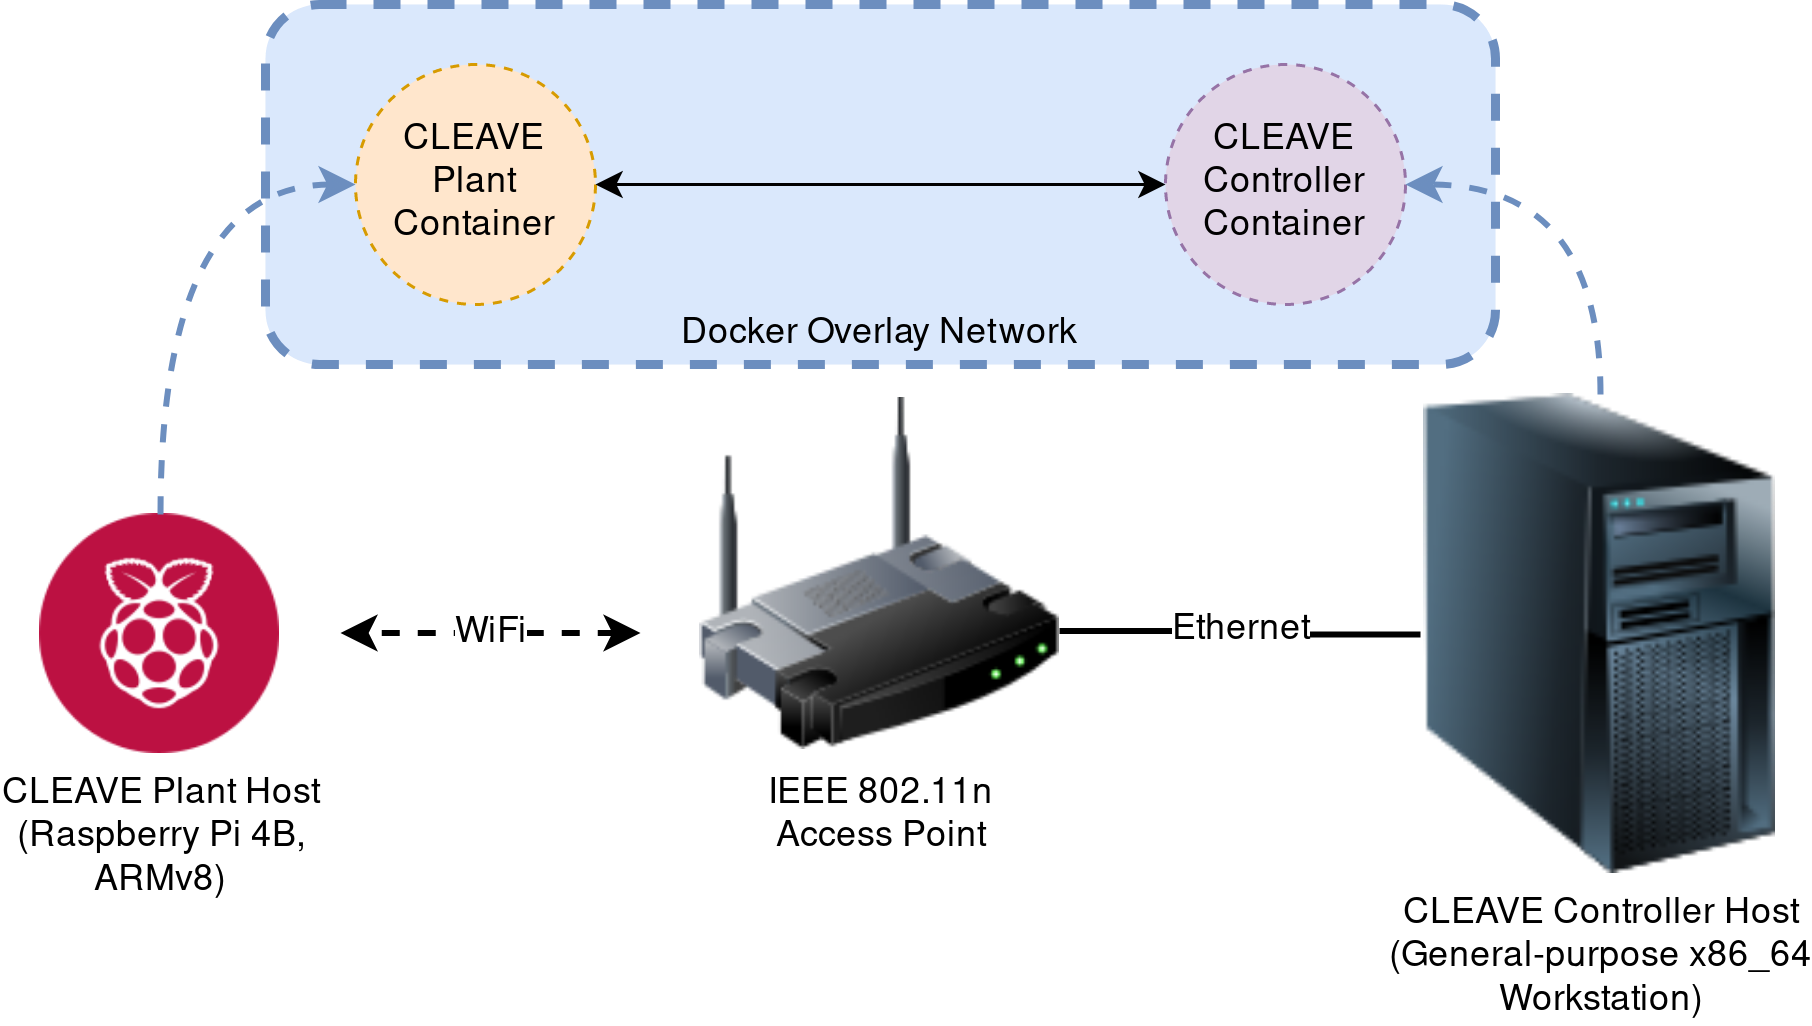
\includegraphics[width=.95\columnwidth]{images/CLEAVE_experiment_setup}
    \caption{Experiment setup}\label{fig:cleave:expsetup}
\end{figure}

In terms of the control system deployed on top of CLEAVE for the experiments, we chose a two-dimensional inverted pendulum system.
This system was chosen due to its relative simplicity and prevalence in the field of automatic control as one of the fundamental examples basically every control engineer has encountered at some point.

The physical system, represented in \cref{fig:invpend}, was implemented using CLEAVE's API and a 2D physics library~\autocite{chipmunk2d,pymunk}.
For the controller, a proportional-differential strategy was employed, implemented using the framework Controller API and the NumPy numeric computation library~\autocite{harris2020array}.

\begin{figure}
    \centering
    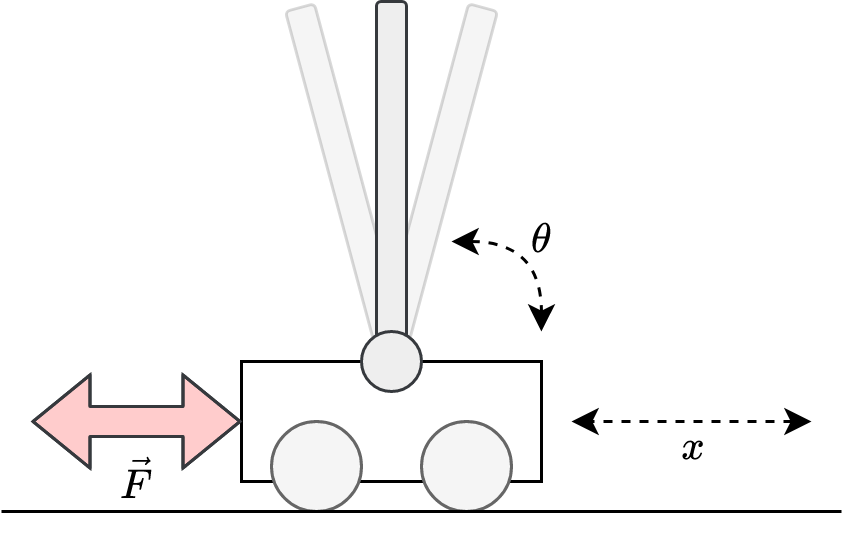
\includegraphics[width=.95\columnwidth]{images/inverted_pendulum.png}
    \caption{
        The two-dimensional inverted pendulum system.
        The cart moves on the X-axis, and the pendulum on top of it swings freely.
        The objective of the system is to balance the pendulum vertically through the application of horizontal forces on the cart.
    }\label{fig:invpend}
\end{figure}